% Options for packages loaded elsewhere
\PassOptionsToPackage{unicode}{hyperref}
\PassOptionsToPackage{hyphens}{url}
%
\documentclass[
]{article}
\usepackage{lmodern}
\usepackage{amssymb,amsmath}
\usepackage{ifxetex,ifluatex}
\ifnum 0\ifxetex 1\fi\ifluatex 1\fi=0 % if pdftex
  \usepackage[T1]{fontenc}
  \usepackage[utf8]{inputenc}
  \usepackage{textcomp} % provide euro and other symbols
\else % if luatex or xetex
  \usepackage{unicode-math}
  \defaultfontfeatures{Scale=MatchLowercase}
  \defaultfontfeatures[\rmfamily]{Ligatures=TeX,Scale=1}
\fi
% Use upquote if available, for straight quotes in verbatim environments
\IfFileExists{upquote.sty}{\usepackage{upquote}}{}
\IfFileExists{microtype.sty}{% use microtype if available
  \usepackage[]{microtype}
  \UseMicrotypeSet[protrusion]{basicmath} % disable protrusion for tt fonts
}{}
\makeatletter
\@ifundefined{KOMAClassName}{% if non-KOMA class
  \IfFileExists{parskip.sty}{%
    \usepackage{parskip}
  }{% else
    \setlength{\parindent}{0pt}
    \setlength{\parskip}{6pt plus 2pt minus 1pt}}
}{% if KOMA class
  \KOMAoptions{parskip=half}}
\makeatother
\usepackage{xcolor}
\IfFileExists{xurl.sty}{\usepackage{xurl}}{} % add URL line breaks if available
\IfFileExists{bookmark.sty}{\usepackage{bookmark}}{\usepackage{hyperref}}
\hypersetup{
  pdftitle={Markov Sick-Sicker model in R},
  pdfauthor={The DARTH workgroup},
  hidelinks,
  pdfcreator={LaTeX via pandoc}}
\urlstyle{same} % disable monospaced font for URLs
\usepackage[margin=1in]{geometry}
\usepackage{color}
\usepackage{fancyvrb}
\newcommand{\VerbBar}{|}
\newcommand{\VERB}{\Verb[commandchars=\\\{\}]}
\DefineVerbatimEnvironment{Highlighting}{Verbatim}{commandchars=\\\{\}}
% Add ',fontsize=\small' for more characters per line
\usepackage{framed}
\definecolor{shadecolor}{RGB}{248,248,248}
\newenvironment{Shaded}{\begin{snugshade}}{\end{snugshade}}
\newcommand{\AlertTok}[1]{\textcolor[rgb]{0.94,0.16,0.16}{#1}}
\newcommand{\AnnotationTok}[1]{\textcolor[rgb]{0.56,0.35,0.01}{\textbf{\textit{#1}}}}
\newcommand{\AttributeTok}[1]{\textcolor[rgb]{0.77,0.63,0.00}{#1}}
\newcommand{\BaseNTok}[1]{\textcolor[rgb]{0.00,0.00,0.81}{#1}}
\newcommand{\BuiltInTok}[1]{#1}
\newcommand{\CharTok}[1]{\textcolor[rgb]{0.31,0.60,0.02}{#1}}
\newcommand{\CommentTok}[1]{\textcolor[rgb]{0.56,0.35,0.01}{\textit{#1}}}
\newcommand{\CommentVarTok}[1]{\textcolor[rgb]{0.56,0.35,0.01}{\textbf{\textit{#1}}}}
\newcommand{\ConstantTok}[1]{\textcolor[rgb]{0.00,0.00,0.00}{#1}}
\newcommand{\ControlFlowTok}[1]{\textcolor[rgb]{0.13,0.29,0.53}{\textbf{#1}}}
\newcommand{\DataTypeTok}[1]{\textcolor[rgb]{0.13,0.29,0.53}{#1}}
\newcommand{\DecValTok}[1]{\textcolor[rgb]{0.00,0.00,0.81}{#1}}
\newcommand{\DocumentationTok}[1]{\textcolor[rgb]{0.56,0.35,0.01}{\textbf{\textit{#1}}}}
\newcommand{\ErrorTok}[1]{\textcolor[rgb]{0.64,0.00,0.00}{\textbf{#1}}}
\newcommand{\ExtensionTok}[1]{#1}
\newcommand{\FloatTok}[1]{\textcolor[rgb]{0.00,0.00,0.81}{#1}}
\newcommand{\FunctionTok}[1]{\textcolor[rgb]{0.00,0.00,0.00}{#1}}
\newcommand{\ImportTok}[1]{#1}
\newcommand{\InformationTok}[1]{\textcolor[rgb]{0.56,0.35,0.01}{\textbf{\textit{#1}}}}
\newcommand{\KeywordTok}[1]{\textcolor[rgb]{0.13,0.29,0.53}{\textbf{#1}}}
\newcommand{\NormalTok}[1]{#1}
\newcommand{\OperatorTok}[1]{\textcolor[rgb]{0.81,0.36,0.00}{\textbf{#1}}}
\newcommand{\OtherTok}[1]{\textcolor[rgb]{0.56,0.35,0.01}{#1}}
\newcommand{\PreprocessorTok}[1]{\textcolor[rgb]{0.56,0.35,0.01}{\textit{#1}}}
\newcommand{\RegionMarkerTok}[1]{#1}
\newcommand{\SpecialCharTok}[1]{\textcolor[rgb]{0.00,0.00,0.00}{#1}}
\newcommand{\SpecialStringTok}[1]{\textcolor[rgb]{0.31,0.60,0.02}{#1}}
\newcommand{\StringTok}[1]{\textcolor[rgb]{0.31,0.60,0.02}{#1}}
\newcommand{\VariableTok}[1]{\textcolor[rgb]{0.00,0.00,0.00}{#1}}
\newcommand{\VerbatimStringTok}[1]{\textcolor[rgb]{0.31,0.60,0.02}{#1}}
\newcommand{\WarningTok}[1]{\textcolor[rgb]{0.56,0.35,0.01}{\textbf{\textit{#1}}}}
\usepackage{graphicx,grffile}
\makeatletter
\def\maxwidth{\ifdim\Gin@nat@width>\linewidth\linewidth\else\Gin@nat@width\fi}
\def\maxheight{\ifdim\Gin@nat@height>\textheight\textheight\else\Gin@nat@height\fi}
\makeatother
% Scale images if necessary, so that they will not overflow the page
% margins by default, and it is still possible to overwrite the defaults
% using explicit options in \includegraphics[width, height, ...]{}
\setkeys{Gin}{width=\maxwidth,height=\maxheight,keepaspectratio}
% Set default figure placement to htbp
\makeatletter
\def\fps@figure{htbp}
\makeatother
\setlength{\emergencystretch}{3em} % prevent overfull lines
\providecommand{\tightlist}{%
  \setlength{\itemsep}{0pt}\setlength{\parskip}{0pt}}
\setcounter{secnumdepth}{-\maxdimen} % remove section numbering

\title{Markov Sick-Sicker model in R}
\usepackage{etoolbox}
\makeatletter
\providecommand{\subtitle}[1]{% add subtitle to \maketitle
  \apptocmd{\@title}{\par {\large #1 \par}}{}{}
}
\makeatother
\subtitle{with dependency for time-since model start AND with state-residency
dependency}
\author{The DARTH workgroup}
\date{}

\begin{document}
\maketitle

Developed by the Decision Analysis in R for Technologies in Health
(DARTH) workgroup:

Fernando Alarid-Escudero, PhD (1)

Eva A. Enns, MS, PhD (2)

M.G. Myriam Hunink, MD, PhD (3,4)

Hawre J. Jalal, MD, PhD (5)

Eline M. Krijkamp, MSc (3)

Petros Pechlivanoglou, PhD (6,7)

Alan Yang, MSc (7)

In collaboration of:

\begin{enumerate}
\def\labelenumi{\arabic{enumi}.}
\tightlist
\item
  Drug Policy Program, Center for Research and Teaching in Economics
  (CIDE) - CONACyT, Aguascalientes, Mexico
\item
  University of Minnesota School of Public Health, Minneapolis, MN, USA
\item
  Erasmus MC, Rotterdam, The Netherlands
\item
  Harvard T.H. Chan School of Public Health, Boston, USA
\item
  University of Pittsburgh Graduate School of Public Health, Pittsburgh,
  PA, USA
\item
  University of Toronto, Toronto ON, Canada
\item
  The Hospital for Sick Children, Toronto ON, Canada
\end{enumerate}

Please cite our publications when using this code:

\begin{itemize}
\item
  Jalal H, Pechlivanoglou P, Krijkamp E, Alarid-Escudero F, Enns E,
  Hunink MG. An Overview of R in Health Decision Sciences. Med Decis
  Making. 2017; 37(3): 735-746.
  \url{https://journals.sagepub.com/doi/abs/10.1177/0272989X16686559}
\item
  Krijkamp EM, Alarid-Escudero F, Enns EA, Jalal HJ, Hunink MGM,
  Pechlivanoglou P. Microsimulation modeling for health decision
  sciences using R: A tutorial. Med Decis Making. 2018;38(3):400--22.
  \url{https://journals.sagepub.com/doi/abs/10.1177/0272989X18754513}
\item
  Krijkamp EM, Alarid-Escudero F, Enns E, Pechlivanoglou P, Hunink MM,
  Jalal H. A Multidimensional Array Representation of State-Transition
  Model Dynamics. Med Decis Making. 2020 Online first.
  \url{https://doi.org/10.1177/0272989X19893973}
\end{itemize}

Copyright 2017, THE HOSPITAL FOR SICK CHILDREN AND THE COLLABORATING
INSTITUTIONS. All rights reserved in Canada, the United States and
worldwide. Copyright, trademarks, trade names and any and all associated
intellectual property are exclusively owned by THE HOSPITAL FOR Sick
CHILDREN and the collaborating institutions. These materials may be
used, reproduced, modified, distributed and adapted with proper
attribution.

\newpage

\begin{Shaded}
\begin{Highlighting}[]
\KeywordTok{rm}\NormalTok{(}\DataTypeTok{list =} \KeywordTok{ls}\NormalTok{())      }\CommentTok{# clear memory (removes all the variables from the workspace)}
\end{Highlighting}
\end{Shaded}

\hypertarget{load-packages}{%
\section{01 Load packages}\label{load-packages}}

\begin{Shaded}
\begin{Highlighting}[]
\ControlFlowTok{if}\NormalTok{ (}\OperatorTok{!}\KeywordTok{require}\NormalTok{(}\StringTok{'pacman'}\NormalTok{)) }\KeywordTok{install.packages}\NormalTok{(}\StringTok{'pacman'}\NormalTok{); }\KeywordTok{library}\NormalTok{(pacman) }\CommentTok{# use this package to conveniently install other packages}
\CommentTok{# load (install if required) packages from CRAN}
\KeywordTok{p_load}\NormalTok{(}\StringTok{"here"}\NormalTok{, }\StringTok{"dplyr"}\NormalTok{, }\StringTok{"devtools"}\NormalTok{, }\StringTok{"scales"}\NormalTok{, }\StringTok{"ellipse"}\NormalTok{, }\StringTok{"ggplot2"}\NormalTok{, }\StringTok{"lazyeval"}\NormalTok{, }\StringTok{"igraph"}\NormalTok{, }\StringTok{"truncnorm"}\NormalTok{, }\StringTok{"ggraph"}\NormalTok{, }\StringTok{"reshape2"}\NormalTok{, }\StringTok{"knitr"}\NormalTok{)                                               }
\CommentTok{# load (install if required) packages from GitHub}
\CommentTok{# install_github("DARTH-git/dampack", force = TRUE) Uncomment if there is a newer version}
\CommentTok{# install_github("DARTH-git/dectree", force = TRUE) Uncomment if there is a newer version}
\KeywordTok{p_load_gh}\NormalTok{(}\StringTok{"DARTH-git/dampack"}\NormalTok{, }\StringTok{"DARTH-git/dectree"}\NormalTok{)}
\end{Highlighting}
\end{Shaded}

\hypertarget{load-functions}{%
\section{02 Load functions}\label{load-functions}}

\begin{Shaded}
\begin{Highlighting}[]
\CommentTok{# no functions required}
\end{Highlighting}
\end{Shaded}

\hypertarget{input-model-parameters}{%
\section{03 Input model parameters}\label{input-model-parameters}}

\begin{Shaded}
\begin{Highlighting}[]
\CommentTok{# Strategy names}
\NormalTok{v_names_str <-}\StringTok{ }\KeywordTok{c}\NormalTok{(}\StringTok{"No Treatment"}\NormalTok{, }\StringTok{"Treatment"}\NormalTok{) }

\CommentTok{# Number of strategies}
\NormalTok{n_str <-}\StringTok{ }\KeywordTok{length}\NormalTok{(v_names_str)}

\CommentTok{# Markov model parameters}
\NormalTok{age     <-}\StringTok{ }\DecValTok{25}                       \CommentTok{# age at baseline}
\NormalTok{max_age <-}\StringTok{ }\DecValTok{55}                       \CommentTok{# maximum age of follow up}
\NormalTok{n_t     <-}\StringTok{ }\NormalTok{max_age }\OperatorTok{-}\StringTok{ }\NormalTok{age            }\CommentTok{# time horizon, number of cycles}
\NormalTok{v_n     <-}\StringTok{ }\KeywordTok{c}\NormalTok{(}\StringTok{"H"}\NormalTok{, }\StringTok{"S1"}\NormalTok{, }\StringTok{"S2"}\NormalTok{, }\StringTok{"D"}\NormalTok{)  }\CommentTok{# the 4 states of the model: Healthy (H), Sick (S1), }
                                    \CommentTok{# Sicker (S2), Dead (D)}
\NormalTok{n_states     <-}\StringTok{ }\KeywordTok{length}\NormalTok{(v_n)         }\CommentTok{# number of health states }

\CommentTok{# Tunnels}
\NormalTok{n_tunnel_size <-}\StringTok{ }\NormalTok{n_t}
\CommentTok{# Sick state}
\NormalTok{v_Sick_tunnels <-}\StringTok{ }\KeywordTok{paste}\NormalTok{(}\StringTok{"S1_"}\NormalTok{, }\KeywordTok{seq}\NormalTok{(}\DecValTok{1}\NormalTok{, n_tunnel_size), }\StringTok{"Yr"}\NormalTok{, }\DataTypeTok{sep =} \StringTok{""}\NormalTok{)}
\CommentTok{### Create variables for time-dependent model}
\NormalTok{v_n_tunnels      <-}\StringTok{ }\KeywordTok{c}\NormalTok{(}\StringTok{"H"}\NormalTok{, v_Sick_tunnels, }\StringTok{"S2"}\NormalTok{, }\StringTok{"D"}\NormalTok{)   }\CommentTok{# state names}
\NormalTok{n_states_tunnels <-}\StringTok{ }\KeywordTok{length}\NormalTok{(v_n_tunnels)                 }\CommentTok{# number of states}

\CommentTok{# Transition probabilities (per cycle) and hazard ratios}
\CommentTok{# Read age-specific mortality rates from csv file}
\NormalTok{lt_usa_}\DecValTok{2005}\NormalTok{ <-}\StringTok{ }\KeywordTok{read.csv}\NormalTok{(}\StringTok{"HMD_USA_Mx_2015.csv"}\NormalTok{)}
\NormalTok{v_r_HD <-}\StringTok{ }\NormalTok{lt_usa_}\DecValTok{2005} \OperatorTok\StringTok{ }
\StringTok{  }\KeywordTok{filter}\NormalTok{(Age }\OperatorTok{>=}\StringTok{ }\NormalTok{age }\OperatorTok{&}\StringTok{ }\NormalTok{Age }\OperatorTok{<=}\StringTok{ }\NormalTok{(max_age}\DecValTok{-1}\NormalTok{)) }\OperatorTok
\StringTok{  }\KeywordTok{select}\NormalTok{(Total) }\OperatorTok
\StringTok{  }\KeywordTok{as.matrix}\NormalTok{()}

\NormalTok{p_HD    <-}\StringTok{ }\DecValTok{1} \OperatorTok{-}\StringTok{ }\KeywordTok{exp}\NormalTok{(}\OperatorTok{-}\StringTok{ }\NormalTok{v_r_HD)         }\CommentTok{# probability to die when healthy}
\NormalTok{p_HS1   <-}\StringTok{ }\FloatTok{0.15}                        \CommentTok{# probability to become sick when healthy}
\NormalTok{p_S1H   <-}\StringTok{ }\FloatTok{0.5}                         \CommentTok{# probability to become healthy when sick}

\CommentTok{# Weibull parameters}
\NormalTok{l       <-}\StringTok{ }\FloatTok{0.08} \CommentTok{# scale}
\NormalTok{g       <-}\StringTok{ }\FloatTok{1.1}  \CommentTok{# shape}
\CommentTok{# Weibull function}
\NormalTok{p_S1S2  <-}\StringTok{ }\NormalTok{l}\OperatorTok{*}\NormalTok{g}\OperatorTok{*}\NormalTok{(}\DecValTok{1}\OperatorTok{:}\NormalTok{n_tunnel_size)}\OperatorTok{^}\NormalTok{\{g}\DecValTok{-1}\NormalTok{\} }\CommentTok{# probability to become sicker when sick }
                                       \CommentTok{# (time-dependent)}

\NormalTok{hr_S1   <-}\StringTok{ }\DecValTok{3}                           \CommentTok{# hazard ratio of death in sick vs healthy}
\NormalTok{hr_S2   <-}\StringTok{ }\DecValTok{10}                          \CommentTok{# hazard ratio of death in sicker vs healthy }
\NormalTok{r_HD    <-}\StringTok{ }\OperatorTok{-}\StringTok{ }\KeywordTok{log}\NormalTok{(}\DecValTok{1} \OperatorTok{-}\StringTok{ }\NormalTok{p_HD)           }\CommentTok{# rate of death in healthy}
\NormalTok{r_S1D   <-}\StringTok{ }\NormalTok{hr_S1 }\OperatorTok{*}\StringTok{ }\NormalTok{r_HD                }\CommentTok{# rate of death in sick}
\NormalTok{r_S2D   <-}\StringTok{ }\NormalTok{hr_S2 }\OperatorTok{*}\StringTok{ }\NormalTok{r_HD                }\CommentTok{# rate of death in sicker}
\NormalTok{p_S1D   <-}\StringTok{ }\DecValTok{1} \OperatorTok{-}\StringTok{ }\KeywordTok{exp}\NormalTok{(}\OperatorTok{-}\NormalTok{r_S1D)           }\CommentTok{# probability to die in sick}
\NormalTok{p_S2D   <-}\StringTok{ }\DecValTok{1} \OperatorTok{-}\StringTok{ }\KeywordTok{exp}\NormalTok{(}\OperatorTok{-}\NormalTok{r_S2D)           }\CommentTok{# probability to die in sicker}

\CommentTok{# Cost and utility inputs    }
\NormalTok{c_H     <-}\StringTok{ }\DecValTok{2000}                      \CommentTok{# cost of remaining one cycle in the healthy state}
\NormalTok{c_S1    <-}\StringTok{ }\DecValTok{4000}                      \CommentTok{# cost of remaining one cycle in the sick state}
\NormalTok{c_S2    <-}\StringTok{ }\DecValTok{15000}                     \CommentTok{# cost of remaining one cycle in the sicker state}
\NormalTok{c_trt   <-}\StringTok{ }\DecValTok{12000}                     \CommentTok{# cost of treatment(per cycle)}
\NormalTok{c_D     <-}\StringTok{ }\DecValTok{0}                         \CommentTok{# cost of being in the death state}
\NormalTok{u_H     <-}\StringTok{ }\DecValTok{1}                         \CommentTok{# utility when healthy}
\NormalTok{u_S1    <-}\StringTok{ }\FloatTok{0.75}                      \CommentTok{# utility when sick}
\NormalTok{u_S2    <-}\StringTok{ }\FloatTok{0.5}                       \CommentTok{# utility when sicker}
\NormalTok{u_D     <-}\StringTok{ }\DecValTok{0}                         \CommentTok{# utility when dead}
\NormalTok{u_trt   <-}\StringTok{ }\FloatTok{0.95}                      \CommentTok{# utility when being treated}

\CommentTok{# Discounting factor}
\NormalTok{d_r     <-}\StringTok{ }\FloatTok{0.03}                      \CommentTok{# equal discount of costs and QALYs by 3%}
\CommentTok{# calculate discount weights for costs for each cycle based on discount rate d_c}
\NormalTok{v_dwc   <-}\StringTok{ }\DecValTok{1} \OperatorTok{/}\StringTok{ }\NormalTok{(}\DecValTok{1} \OperatorTok{+}\StringTok{ }\NormalTok{d_r) }\OperatorTok{^}\StringTok{ }\NormalTok{(}\DecValTok{0}\OperatorTok{:}\NormalTok{n_t) }
\CommentTok{# calculate discount weights for effectiveness for each cycle based on discount rate d_e}
\NormalTok{v_dwe   <-}\StringTok{ }\DecValTok{1} \OperatorTok{/}\StringTok{ }\NormalTok{(}\DecValTok{1} \OperatorTok{+}\StringTok{ }\NormalTok{d_r) }\OperatorTok{^}\StringTok{ }\NormalTok{(}\DecValTok{0}\OperatorTok{:}\NormalTok{n_t) }
\end{Highlighting}
\end{Shaded}

\hypertarget{define-and-initialize-matrices-and-vectors}{%
\section{04 Define and initialize matrices and
vectors}\label{define-and-initialize-matrices-and-vectors}}

\hypertarget{cohort-trace}{%
\subsection{04.1 Cohort trace}\label{cohort-trace}}

\begin{Shaded}
\begin{Highlighting}[]
\CommentTok{# create the markov trace matrix M capturing the proportion of the cohort in each state }
\CommentTok{# at each cycle}
\NormalTok{m_M_notrt <-}\StringTok{ }\NormalTok{m_M_trt <-}\StringTok{ }\KeywordTok{matrix}\NormalTok{(}\OtherTok{NA}\NormalTok{, }
                               \DataTypeTok{nrow =}\NormalTok{ n_t }\OperatorTok{+}\StringTok{ }\DecValTok{1}\NormalTok{, }\DataTypeTok{ncol =}\NormalTok{ n_states_tunnels,}
                               \DataTypeTok{dimnames =} \KeywordTok{list}\NormalTok{(}\KeywordTok{paste}\NormalTok{(}\StringTok{"cycle"}\NormalTok{, }\DecValTok{0}\OperatorTok{:}\NormalTok{n_t, }\DataTypeTok{sep =} \StringTok{" "}\NormalTok{), v_n_tunnels)) }

\KeywordTok{head}\NormalTok{(m_M_notrt) }\CommentTok{# show first 6 rows of the matrix }
\end{Highlighting}
\end{Shaded}

\begin{verbatim}
##          H S1_1Yr S1_2Yr S1_3Yr S1_4Yr S1_5Yr S1_6Yr S1_7Yr S1_8Yr S1_9Yr
## cycle 0 NA     NA     NA     NA     NA     NA     NA     NA     NA     NA
## cycle 1 NA     NA     NA     NA     NA     NA     NA     NA     NA     NA
## cycle 2 NA     NA     NA     NA     NA     NA     NA     NA     NA     NA
## cycle 3 NA     NA     NA     NA     NA     NA     NA     NA     NA     NA
## cycle 4 NA     NA     NA     NA     NA     NA     NA     NA     NA     NA
## cycle 5 NA     NA     NA     NA     NA     NA     NA     NA     NA     NA
##         S1_10Yr S1_11Yr S1_12Yr S1_13Yr S1_14Yr S1_15Yr S1_16Yr S1_17Yr S1_18Yr
## cycle 0      NA      NA      NA      NA      NA      NA      NA      NA      NA
## cycle 1      NA      NA      NA      NA      NA      NA      NA      NA      NA
## cycle 2      NA      NA      NA      NA      NA      NA      NA      NA      NA
## cycle 3      NA      NA      NA      NA      NA      NA      NA      NA      NA
## cycle 4      NA      NA      NA      NA      NA      NA      NA      NA      NA
## cycle 5      NA      NA      NA      NA      NA      NA      NA      NA      NA
##         S1_19Yr S1_20Yr S1_21Yr S1_22Yr S1_23Yr S1_24Yr S1_25Yr S1_26Yr S1_27Yr
## cycle 0      NA      NA      NA      NA      NA      NA      NA      NA      NA
## cycle 1      NA      NA      NA      NA      NA      NA      NA      NA      NA
## cycle 2      NA      NA      NA      NA      NA      NA      NA      NA      NA
## cycle 3      NA      NA      NA      NA      NA      NA      NA      NA      NA
## cycle 4      NA      NA      NA      NA      NA      NA      NA      NA      NA
## cycle 5      NA      NA      NA      NA      NA      NA      NA      NA      NA
##         S1_28Yr S1_29Yr S1_30Yr S2  D
## cycle 0      NA      NA      NA NA NA
## cycle 1      NA      NA      NA NA NA
## cycle 2      NA      NA      NA NA NA
## cycle 3      NA      NA      NA NA NA
## cycle 4      NA      NA      NA NA NA
## cycle 5      NA      NA      NA NA NA
\end{verbatim}

\begin{Shaded}
\begin{Highlighting}[]
\CommentTok{# The cohort starts as healthy}
\CommentTok{# initialize first cycle of Markov trace accounting for the tunnels}
\NormalTok{m_M_notrt[}\DecValTok{1}\NormalTok{, ] <-}\StringTok{ }\NormalTok{m_M_trt[}\DecValTok{1}\NormalTok{, ] <-}\StringTok{ }\KeywordTok{c}\NormalTok{(}\DecValTok{1}\NormalTok{, }\KeywordTok{rep}\NormalTok{(}\DecValTok{0}\NormalTok{, n_tunnel_size), }\DecValTok{0}\NormalTok{, }\DecValTok{0}\NormalTok{) }
\end{Highlighting}
\end{Shaded}

\hypertarget{transition-probability-array}{%
\subsection{04.2 Transition probability
array}\label{transition-probability-array}}

\begin{Shaded}
\begin{Highlighting}[]
\CommentTok{# create the transition probability array for NO treatment}
\NormalTok{a_P_notrt <-}\StringTok{ }\KeywordTok{array}\NormalTok{(}\DecValTok{0}\NormalTok{,                                          }\CommentTok{# Create 3-D array}
                   \DataTypeTok{dim =} \KeywordTok{c}\NormalTok{(n_states_tunnels, n_states_tunnels, n_t),}
                   \DataTypeTok{dimnames =} \KeywordTok{list}\NormalTok{(v_n_tunnels, v_n_tunnels, }\DecValTok{0}\OperatorTok{:}\NormalTok{(n_t}\DecValTok{-1}\NormalTok{))) }\CommentTok{# name dimensions}
\end{Highlighting}
\end{Shaded}

Fill in the transition probability array:

\begin{Shaded}
\begin{Highlighting}[]
\CommentTok{# from Healthy}
\NormalTok{a_P_notrt[}\StringTok{"H"}\NormalTok{, }\StringTok{"H"}\NormalTok{, ]               <-}\StringTok{ }\DecValTok{1} \OperatorTok{-}\StringTok{ }\NormalTok{(p_HS1 }\OperatorTok{+}\StringTok{ }\NormalTok{p_HD)}
\NormalTok{a_P_notrt[}\StringTok{"H"}\NormalTok{, v_Sick_tunnels[}\DecValTok{1}\NormalTok{], ] <-}\StringTok{ }\NormalTok{p_HS1}
\NormalTok{a_P_notrt[}\StringTok{"H"}\NormalTok{, }\StringTok{"D"}\NormalTok{, ]               <-}\StringTok{ }\NormalTok{p_HD}

\CommentTok{# from Sick}
\ControlFlowTok{for}\NormalTok{(i }\ControlFlowTok{in} \DecValTok{1}\OperatorTok{:}\NormalTok{(n_tunnel_size }\OperatorTok{-}\StringTok{ }\DecValTok{1}\NormalTok{))\{}
\NormalTok{  a_P_notrt[v_Sick_tunnels[i], }\StringTok{"H"}\NormalTok{, ]  <-}\StringTok{ }\NormalTok{p_S1H}
\NormalTok{  a_P_notrt[v_Sick_tunnels[i], v_Sick_tunnels[i }\OperatorTok{+}\StringTok{ }\DecValTok{1}\NormalTok{], ] <-}\StringTok{ }\DecValTok{1} \OperatorTok{-}\StringTok{ }\NormalTok{(p_S1H }\OperatorTok{+}\StringTok{ }\NormalTok{p_S1S2[i] }\OperatorTok{+}\StringTok{ }\NormalTok{p_S1D)}
\NormalTok{  a_P_notrt[v_Sick_tunnels[i], }\StringTok{"S2"}\NormalTok{, ] <-}\StringTok{ }\NormalTok{p_S1S2[i]}
\NormalTok{  a_P_notrt[v_Sick_tunnels[i], }\StringTok{"D"}\NormalTok{, ]  <-}\StringTok{ }\NormalTok{p_S1D}
\NormalTok{\}}
\NormalTok{a_P_notrt[v_Sick_tunnels[n_tunnel_size], }\StringTok{"H"}\NormalTok{, ]  <-}\StringTok{ }\NormalTok{p_S1H}
\NormalTok{a_P_notrt[v_Sick_tunnels[n_tunnel_size], v_Sick_tunnels[n_tunnel_size], ] <-}\StringTok{ }\DecValTok{1} \OperatorTok{-}\StringTok{ }
\StringTok{         }\NormalTok{(p_S1H }\OperatorTok{+}\StringTok{ }\NormalTok{p_S1S2[n_tunnel_size] }\OperatorTok{+}\StringTok{ }\NormalTok{p_S1D)}
\NormalTok{a_P_notrt[v_Sick_tunnels[n_tunnel_size], }\StringTok{"S2"}\NormalTok{, ] <-}\StringTok{ }\NormalTok{p_S1S2[n_tunnel_size]}
\NormalTok{a_P_notrt[v_Sick_tunnels[n_tunnel_size], }\StringTok{"D"}\NormalTok{, ]  <-}\StringTok{ }\NormalTok{p_S1D}

\CommentTok{# from Sicker}
\NormalTok{a_P_notrt[}\StringTok{"S2"}\NormalTok{, }\StringTok{"S2"}\NormalTok{, ] <-}\StringTok{ }\DecValTok{1} \OperatorTok{-}\StringTok{ }\NormalTok{p_S2D}
\NormalTok{a_P_notrt[}\StringTok{"S2"}\NormalTok{, }\StringTok{"D"}\NormalTok{, ]  <-}\StringTok{ }\NormalTok{p_S2D}

\CommentTok{# from Dead}
\NormalTok{a_P_notrt[}\StringTok{"D"}\NormalTok{, }\StringTok{"D"}\NormalTok{, ]   <-}\StringTok{ }\DecValTok{1}

\CommentTok{# Check if transition matrix is valid (i_e_, each row should add up to 1)}
\NormalTok{valid <-}\StringTok{ }\KeywordTok{apply}\NormalTok{(a_P_notrt, }\DecValTok{3}\NormalTok{, }\ControlFlowTok{function}\NormalTok{(x) }\KeywordTok{sum}\NormalTok{(}\KeywordTok{rowSums}\NormalTok{(x))}\OperatorTok{==}\NormalTok{n_states_tunnels)}
\ControlFlowTok{if}\NormalTok{ (}\OperatorTok{!}\KeywordTok{isTRUE}\NormalTok{(}\KeywordTok{all.equal}\NormalTok{(}\KeywordTok{as.numeric}\NormalTok{(}\KeywordTok{sum}\NormalTok{(valid)), }\KeywordTok{as.numeric}\NormalTok{(n_t)))) \{}
  \KeywordTok{stop}\NormalTok{(}\StringTok{"This is not a valid transition Matrix"}\NormalTok{)}
\NormalTok{\}}

\CommentTok{# create transition probability matrix for treatment same as NO treatment}
\NormalTok{a_P_trt <-}\StringTok{ }\NormalTok{a_P_notrt}
\end{Highlighting}
\end{Shaded}

\hypertarget{run-markov-model}{%
\section{05 Run Markov model}\label{run-markov-model}}

\begin{Shaded}
\begin{Highlighting}[]
\ControlFlowTok{for}\NormalTok{ (t }\ControlFlowTok{in} \DecValTok{1}\OperatorTok{:}\NormalTok{n_t)\{   }\CommentTok{# loop through the number of cycles}
\NormalTok{  m_M_notrt[t }\OperatorTok{+}\StringTok{ }\DecValTok{1}\NormalTok{, ] <-}\StringTok{ }\KeywordTok{t}\NormalTok{(m_M_notrt[t, ]) }\OperatorTok\StringTok{ }\NormalTok{a_P_notrt[ , , t]     }\CommentTok{# estimate the Markov }
                                                                    \CommentTok{# trace for cycle the }
                                                                    \CommentTok{# next cycle (t + 1)}
  
\NormalTok{  m_M_trt[t }\OperatorTok{+}\StringTok{ }\DecValTok{1}\NormalTok{, ]   <-}\StringTok{ }\KeywordTok{t}\NormalTok{(m_M_trt[t, ])   }\OperatorTok\StringTok{ }\NormalTok{a_P_trt[, , t]        }\CommentTok{# estimate the Markov }
                                                                    \CommentTok{# trace for cycle the }
                                                                    \CommentTok{# next cycle (t + 1)}
\NormalTok{\} }\CommentTok{# close the loop}

\KeywordTok{head}\NormalTok{(m_M_notrt)  }\CommentTok{# show the first 6 lines of the matrix}
\end{Highlighting}
\end{Shaded}

\begin{verbatim}
##                 H    S1_1Yr     S1_2Yr     S1_3Yr      S1_4Yr      S1_5Yr
## cycle 0 1.0000000 0.0000000 0.00000000 0.00000000 0.000000000 0.000000000
## cycle 1 0.8489865 0.1500000 0.00000000 0.00000000 0.000000000 0.000000000
## cycle 2 0.7957908 0.1273480 0.06135112 0.00000000 0.000000000 0.000000000
## cycle 3 0.7699207 0.1193686 0.05205923 0.02469254 0.000000000 0.000000000
## cycle 4 0.7516564 0.1154881 0.04879125 0.02095011 0.009840608 0.000000000
## cycle 5 0.7355700 0.1127485 0.04717921 0.01962403 0.008344453 0.003891317
##         S1_6Yr S1_7Yr S1_8Yr S1_9Yr S1_10Yr S1_11Yr S1_12Yr S1_13Yr S1_14Yr
## cycle 0      0      0      0      0       0       0       0       0       0
## cycle 1      0      0      0      0       0       0       0       0       0
## cycle 2      0      0      0      0       0       0       0       0       0
## cycle 3      0      0      0      0       0       0       0       0       0
## cycle 4      0      0      0      0       0       0       0       0       0
## cycle 5      0      0      0      0       0       0       0       0       0
##         S1_15Yr S1_16Yr S1_17Yr S1_18Yr S1_19Yr S1_20Yr S1_21Yr S1_22Yr S1_23Yr
## cycle 0       0       0       0       0       0       0       0       0       0
## cycle 1       0       0       0       0       0       0       0       0       0
## cycle 2       0       0       0       0       0       0       0       0       0
## cycle 3       0       0       0       0       0       0       0       0       0
## cycle 4       0       0       0       0       0       0       0       0       0
## cycle 5       0       0       0       0       0       0       0       0       0
##         S1_24Yr S1_25Yr S1_26Yr S1_27Yr S1_28Yr S1_29Yr S1_30Yr         S2
## cycle 0       0       0       0       0       0       0       0 0.00000000
## cycle 1       0       0       0       0       0       0       0 0.00000000
## cycle 2       0       0       0       0       0       0       0 0.01320000
## cycle 3       0       0       0       0       0       0       0 0.03005253
## cycle 4       0       0       0       0       0       0       0 0.04756736
## cycle 5       0       0       0       0       0       0       0 0.06483502
##                   D
## cycle 0 0.000000000
## cycle 1 0.001013486
## cycle 2 0.002310077
## cycle 3 0.003906358
## cycle 4 0.005706216
## cycle 5 0.007807498
\end{verbatim}

\begin{Shaded}
\begin{Highlighting}[]
\CommentTok{# create aggregated traces}
\NormalTok{m_M_td_notrt <-}\StringTok{ }\KeywordTok{cbind}\NormalTok{(}\DataTypeTok{H =}\NormalTok{ m_M_notrt[, }\StringTok{"H"}\NormalTok{], }
                      \DataTypeTok{S1 =} \KeywordTok{rowSums}\NormalTok{(m_M_notrt[, }\DecValTok{2}\OperatorTok{:}\NormalTok{(n_tunnel_size }\OperatorTok{+}\DecValTok{1}\NormalTok{)]), }
                      \DataTypeTok{S2 =}\NormalTok{ m_M_notrt[, }\StringTok{"S2"}\NormalTok{],}
                      \DataTypeTok{D =}\NormalTok{ m_M_notrt[, }\StringTok{"D"}\NormalTok{])}
\KeywordTok{head}\NormalTok{(m_M_td_notrt)}
\end{Highlighting}
\end{Shaded}

\begin{verbatim}
##                 H        S1         S2           D
## cycle 0 1.0000000 0.0000000 0.00000000 0.000000000
## cycle 1 0.8489865 0.1500000 0.00000000 0.001013486
## cycle 2 0.7957908 0.1886991 0.01320000 0.002310077
## cycle 3 0.7699207 0.1961204 0.03005253 0.003906358
## cycle 4 0.7516564 0.1950701 0.04756736 0.005706216
## cycle 5 0.7355700 0.1917875 0.06483502 0.007807498
\end{verbatim}

\begin{Shaded}
\begin{Highlighting}[]
\NormalTok{m_M_td_trt   <-}\StringTok{ }\KeywordTok{cbind}\NormalTok{(}\DataTypeTok{H =}\NormalTok{ m_M_trt[, }\StringTok{"H"}\NormalTok{], }
                      \DataTypeTok{S1 =} \KeywordTok{rowSums}\NormalTok{(m_M_trt[, }\DecValTok{2}\OperatorTok{:}\NormalTok{(n_tunnel_size }\OperatorTok{+}\DecValTok{1}\NormalTok{)]), }
                      \DataTypeTok{S2 =}\NormalTok{ m_M_trt[, }\StringTok{"S2"}\NormalTok{],}
                      \DataTypeTok{D =}\NormalTok{ m_M_trt[, }\StringTok{"D"}\NormalTok{])}
\KeywordTok{head}\NormalTok{(m_M_td_trt)}
\end{Highlighting}
\end{Shaded}

\begin{verbatim}
##                 H        S1         S2           D
## cycle 0 1.0000000 0.0000000 0.00000000 0.000000000
## cycle 1 0.8489865 0.1500000 0.00000000 0.001013486
## cycle 2 0.7957908 0.1886991 0.01320000 0.002310077
## cycle 3 0.7699207 0.1961204 0.03005253 0.003906358
## cycle 4 0.7516564 0.1950701 0.04756736 0.005706216
## cycle 5 0.7355700 0.1917875 0.06483502 0.007807498
\end{verbatim}

\hypertarget{compute-and-plot-epidemiological-outcomes}{%
\section{06 Compute and Plot Epidemiological
Outcomes}\label{compute-and-plot-epidemiological-outcomes}}

\hypertarget{cohort-trace-1}{%
\subsection{06.1 Cohort trace}\label{cohort-trace-1}}

\begin{Shaded}
\begin{Highlighting}[]
\CommentTok{# create a plot of the data}
\KeywordTok{matplot}\NormalTok{(m_M_td_notrt, }\DataTypeTok{type =} \StringTok{'l'}\NormalTok{, }
        \DataTypeTok{ylab =} \StringTok{"Probability of state occupancy"}\NormalTok{,}
        \DataTypeTok{xlab =} \StringTok{"Cycle"}\NormalTok{,}
        \DataTypeTok{main =} \StringTok{"Cohort Trace"}\NormalTok{)                 }
\CommentTok{# add a legend to the graph}
\KeywordTok{legend}\NormalTok{(}\StringTok{"topright"}\NormalTok{, v_n, }\DataTypeTok{col =} \DecValTok{1}\OperatorTok{:}\NormalTok{n_states,}\DataTypeTok{lty =} \DecValTok{1}\OperatorTok{:}\NormalTok{n_states, }\DataTypeTok{bty =} \StringTok{"n"}\NormalTok{) }
\end{Highlighting}
\end{Shaded}

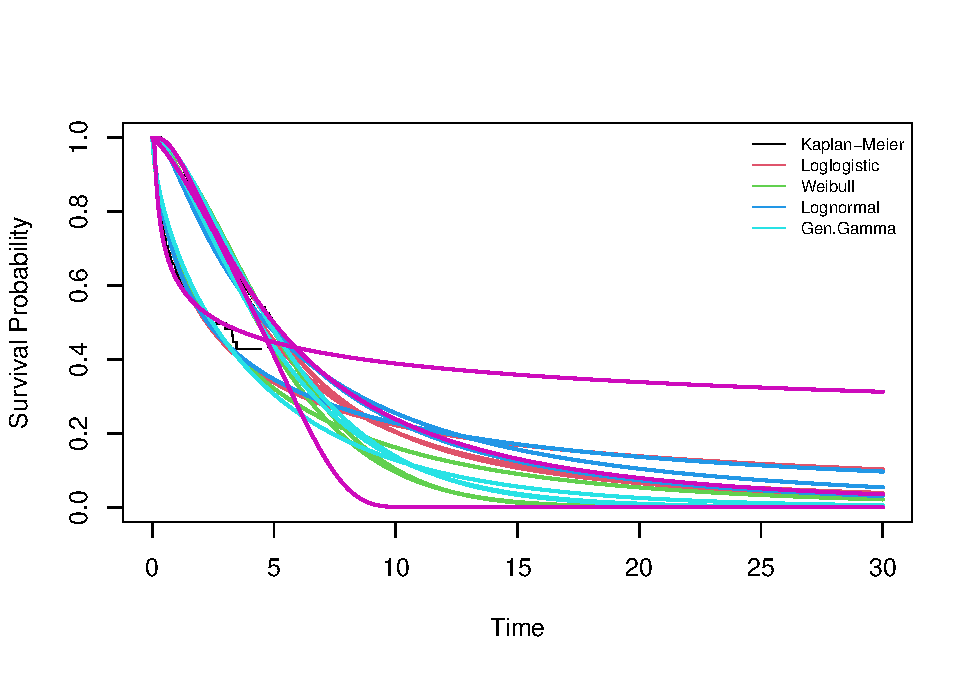
\includegraphics{markov_sick-sicker_tunnels_solutions_files/figure-latex/unnamed-chunk-9-1.pdf}

\hypertarget{overall-survival-os}{%
\subsection{06.2 Overall Survival (OS)}\label{overall-survival-os}}

\begin{Shaded}
\begin{Highlighting}[]
\CommentTok{# calculate the overall survival (OS) probability for no treatment}
\NormalTok{v_os_notrt_tunnels <-}\StringTok{ }\DecValTok{1} \OperatorTok{-}\StringTok{ }\NormalTok{m_M_notrt[, }\StringTok{"D"}\NormalTok{]       }
\CommentTok{# alternative way of calculating the OS probability }
\NormalTok{v_os_notrt_tunnels <-}\StringTok{ }\KeywordTok{rowSums}\NormalTok{(m_M_notrt[, }\DecValTok{1}\OperatorTok{:}\DecValTok{3}\NormalTok{])    }
\CommentTok{# create a simple plot showing the OS}
\KeywordTok{plot}\NormalTok{(age}\OperatorTok{:}\NormalTok{max_age, v_os_notrt_tunnels, }\DataTypeTok{type =} \StringTok{'l'}\NormalTok{, }
     \DataTypeTok{ylim =} \KeywordTok{c}\NormalTok{(}\DecValTok{0}\NormalTok{, }\DecValTok{1}\NormalTok{),}
     \DataTypeTok{ylab =} \StringTok{"Survival probability"}\NormalTok{,}
     \DataTypeTok{xlab =} \StringTok{"Age"}\NormalTok{,}
     \DataTypeTok{main =} \StringTok{"Overall Survival Age-dependent with tunnels"}\NormalTok{)  }
\CommentTok{# add grid }
\KeywordTok{grid}\NormalTok{(}\DataTypeTok{nx =}\NormalTok{ n_t, }\DataTypeTok{ny =} \DecValTok{10}\NormalTok{, }\DataTypeTok{col =} \StringTok{"lightgray"}\NormalTok{, }\DataTypeTok{lty =} \StringTok{"dotted"}\NormalTok{, }\DataTypeTok{lwd =} \KeywordTok{par}\NormalTok{(}\StringTok{"lwd"}\NormalTok{), }
     \DataTypeTok{equilogs =} \OtherTok{TRUE}\NormalTok{) }
\end{Highlighting}
\end{Shaded}

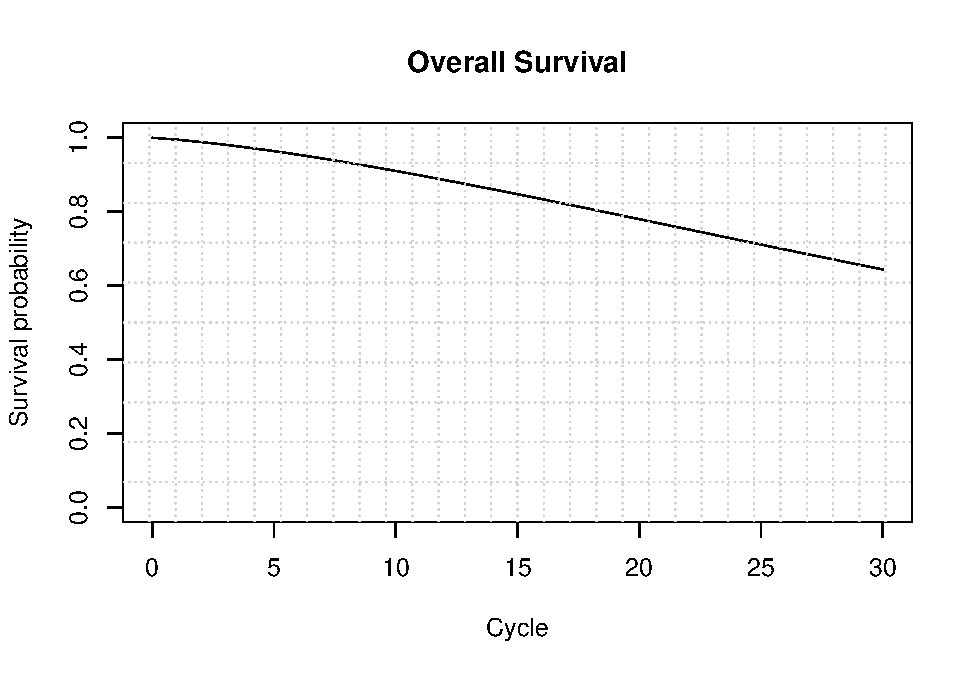
\includegraphics{markov_sick-sicker_tunnels_solutions_files/figure-latex/unnamed-chunk-10-1.pdf}

\hypertarget{life-expectancy-le}{%
\subsection{06.2.1 Life Expectancy (LE)}\label{life-expectancy-le}}

\begin{Shaded}
\begin{Highlighting}[]
\NormalTok{v_le_tunnels <-}\StringTok{ }\KeywordTok{sum}\NormalTok{(v_os_notrt_tunnels)  }\CommentTok{# summing probablity of OS over time }
                                         \CommentTok{# (i_e_ life expectancy)}
\end{Highlighting}
\end{Shaded}

\hypertarget{disease-prevalence}{%
\subsection{06.3 Disease prevalence}\label{disease-prevalence}}

\begin{Shaded}
\begin{Highlighting}[]
\NormalTok{v_prev_tunnels <-}\StringTok{ }\KeywordTok{rowSums}\NormalTok{(m_M_td_notrt[, }\KeywordTok{c}\NormalTok{(}\StringTok{"S1"}\NormalTok{, }\StringTok{"S2"}\NormalTok{)]) }\OperatorTok{/}\StringTok{ }\NormalTok{v_os_notrt_tunnels}
\KeywordTok{plot}\NormalTok{(v_prev_tunnels,}
     \DataTypeTok{ylim =} \KeywordTok{c}\NormalTok{(}\DecValTok{0}\NormalTok{, }\DecValTok{1}\NormalTok{),}
     \DataTypeTok{ylab =} \StringTok{"Prevalence"}\NormalTok{,}
     \DataTypeTok{xlab =} \StringTok{"Cycle"}\NormalTok{,}
     \DataTypeTok{main =} \StringTok{"Disease prevalence"}\NormalTok{)}
\end{Highlighting}
\end{Shaded}

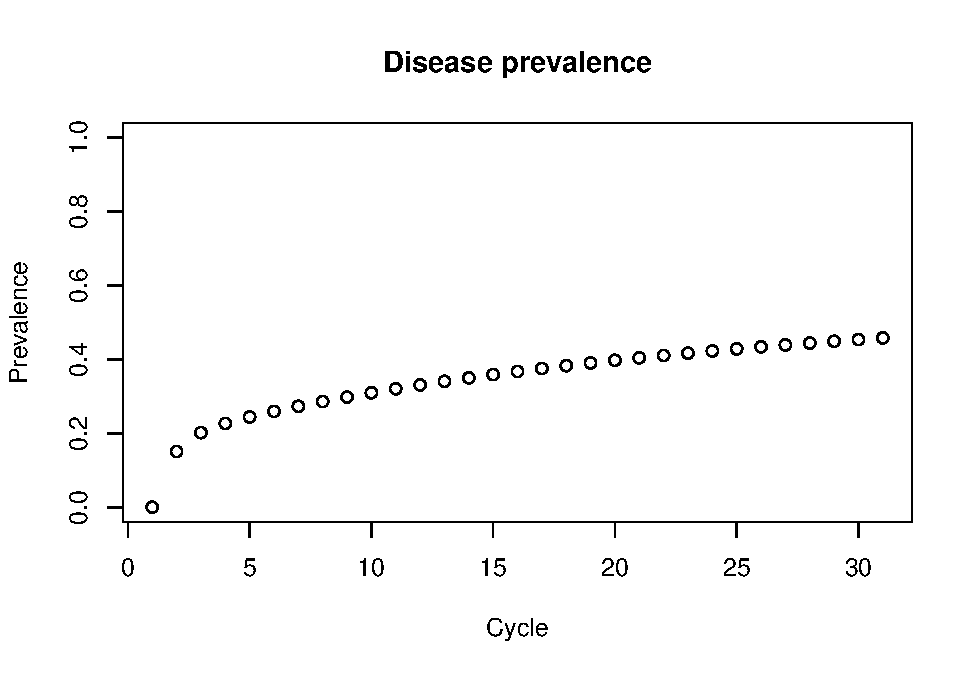
\includegraphics{markov_sick-sicker_tunnels_solutions_files/figure-latex/unnamed-chunk-12-1.pdf}

\hypertarget{ratio-of-sicks1-vs-sickers2}{%
\subsection{06.4 ratio of sick(S1) vs
sicker(S2)}\label{ratio-of-sicks1-vs-sickers2}}

\begin{Shaded}
\begin{Highlighting}[]
\NormalTok{v_ratio_S1S2_tunnels <-}\StringTok{ }\NormalTok{m_M_td_notrt[, }\StringTok{"S1"}\NormalTok{] }\OperatorTok{/}\StringTok{ }\NormalTok{m_M_td_notrt[, }\StringTok{"S2"}\NormalTok{]}
\KeywordTok{plot}\NormalTok{(}\DecValTok{0}\OperatorTok{:}\NormalTok{n_t, v_ratio_S1S2_tunnels,}
     \DataTypeTok{xlab =} \StringTok{"Cycle"}\NormalTok{, }
     \DataTypeTok{ylab =} \StringTok{"Ratio S1 vs S2"}\NormalTok{, }
     \DataTypeTok{main =} \StringTok{"Ratio of sick and sicker"}\NormalTok{, }
     \DataTypeTok{col  =} \StringTok{"black"}\NormalTok{, }\DataTypeTok{type =} \StringTok{"l"}\NormalTok{)}
\end{Highlighting}
\end{Shaded}

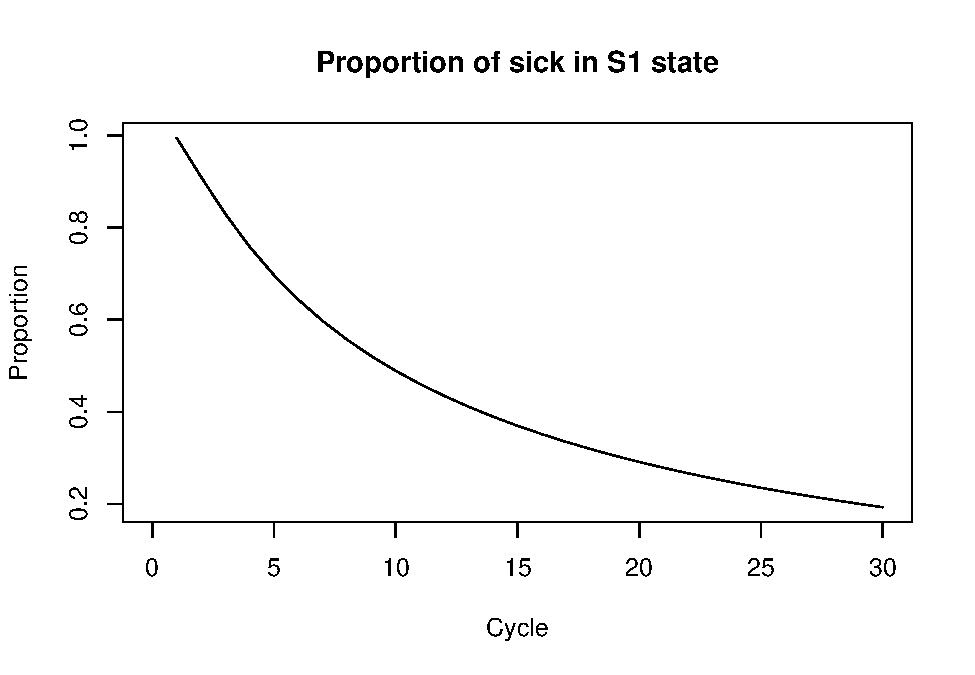
\includegraphics{markov_sick-sicker_tunnels_solutions_files/figure-latex/unnamed-chunk-13-1.pdf}

\hypertarget{compute-cost-effectiveness-outcomes}{%
\section{07 Compute Cost-Effectiveness
Outcomes}\label{compute-cost-effectiveness-outcomes}}

\begin{Shaded}
\begin{Highlighting}[]
\CommentTok{# Vectors with costs and utilities by treatment}
\NormalTok{v_u_notrt   <-}\StringTok{ }\KeywordTok{c}\NormalTok{(u_H, u_S1, u_S2, u_D)}
\NormalTok{v_u_trt     <-}\StringTok{ }\KeywordTok{c}\NormalTok{(u_H, u_trt, u_S2, u_D)}

\NormalTok{v_c_notrt   <-}\StringTok{ }\KeywordTok{c}\NormalTok{(c_H, c_S1, c_S2, c_D)}
\NormalTok{v_c_trt     <-}\StringTok{ }\KeywordTok{c}\NormalTok{(c_H, c_S1 }\OperatorTok{+}\StringTok{ }\NormalTok{c_trt, c_S2 }\OperatorTok{+}\StringTok{ }\NormalTok{c_trt, c_D)}
\end{Highlighting}
\end{Shaded}

\hypertarget{mean-costs-and-qalys-for-treatment-and-no-treatment}{%
\subsection{07.1 Mean Costs and QALYs for Treatment and NO
Treatment}\label{mean-costs-and-qalys-for-treatment-and-no-treatment}}

\begin{Shaded}
\begin{Highlighting}[]
\NormalTok{v_tu_notrt  <-}\StringTok{ }\NormalTok{m_M_td_notrt   }\OperatorTok\StringTok{  }\NormalTok{v_u_notrt}
\NormalTok{v_tu_trt    <-}\StringTok{ }\NormalTok{m_M_td_trt     }\OperatorTok\StringTok{  }\NormalTok{v_u_trt}

\NormalTok{v_tc_notrt  <-}\StringTok{ }\NormalTok{m_M_td_notrt   }\OperatorTok\StringTok{  }\NormalTok{v_c_notrt}
\NormalTok{v_tc_trt    <-}\StringTok{ }\NormalTok{m_M_td_trt     }\OperatorTok\StringTok{  }\NormalTok{v_c_trt}
\end{Highlighting}
\end{Shaded}

\hypertarget{discounted-mean-costs-and-qalys}{%
\subsection{07.2 Discounted Mean Costs and
QALYs}\label{discounted-mean-costs-and-qalys}}

\begin{Shaded}
\begin{Highlighting}[]
\NormalTok{tu_d_notrt  <-}\StringTok{ }\KeywordTok{t}\NormalTok{(v_tu_notrt)  }\OperatorTok\StringTok{  }\NormalTok{v_dwe   }
\NormalTok{tu_d_trt    <-}\StringTok{ }\KeywordTok{t}\NormalTok{(v_tu_trt)    }\OperatorTok\StringTok{  }\NormalTok{v_dwe}

\NormalTok{tc_d_notrt  <-}\StringTok{ }\KeywordTok{t}\NormalTok{(v_tc_notrt)  }\OperatorTok\StringTok{  }\NormalTok{v_dwc}
\NormalTok{tc_d_trt    <-}\StringTok{ }\KeywordTok{t}\NormalTok{(v_tc_trt)    }\OperatorTok\StringTok{  }\NormalTok{v_dwc}


\CommentTok{# store them into a vector}
\NormalTok{v_tc_d      <-}\StringTok{ }\KeywordTok{c}\NormalTok{(tc_d_notrt, tc_d_trt)}
\NormalTok{v_tu_d      <-}\StringTok{ }\KeywordTok{c}\NormalTok{(tu_d_notrt, tu_d_trt)}

\CommentTok{# Dataframe with discounted costs and effectiveness}
\NormalTok{df_ce       <-}\StringTok{ }\KeywordTok{data.frame}\NormalTok{(}\DataTypeTok{Strategy =}\NormalTok{ v_names_str,}
                          \DataTypeTok{Cost     =}\NormalTok{ v_tc_d,}
                          \DataTypeTok{Effect   =}\NormalTok{ v_tu_d)}
\NormalTok{df_ce}
\end{Highlighting}
\end{Shaded}

\begin{verbatim}
##       Strategy      Cost   Effect
## 1 No Treatment  86195.11 17.21135
## 2    Treatment 161264.59 17.83411
\end{verbatim}

\hypertarget{compute-icers-of-the-markov-model}{%
\subsection{07.3 Compute ICERs of the Markov
model}\label{compute-icers-of-the-markov-model}}

\begin{Shaded}
\begin{Highlighting}[]
\NormalTok{df_cea <-}\StringTok{ }\KeywordTok{calculate_icers}\NormalTok{(}\DataTypeTok{cost       =}\NormalTok{ df_ce}\OperatorTok{$}\NormalTok{Cost,}
                          \DataTypeTok{effect     =}\NormalTok{ df_ce}\OperatorTok{$}\NormalTok{Effect,}
                          \DataTypeTok{strategies =}\NormalTok{ df_ce}\OperatorTok{$}\NormalTok{Strategy)}
\NormalTok{df_cea }
\end{Highlighting}
\end{Shaded}

\begin{verbatim}
##       Strategy      Cost   Effect Inc_Cost Inc_Effect     ICER Status
## 1 No Treatment  86195.11 17.21135       NA         NA       NA     ND
## 2    Treatment 161264.59 17.83411 75069.48   0.622759 120543.4     ND
\end{verbatim}

\hypertarget{plot-frontier-of-the-markov-model}{%
\subsection{07.4 Plot frontier of the Markov
model}\label{plot-frontier-of-the-markov-model}}

\begin{Shaded}
\begin{Highlighting}[]
\KeywordTok{plot}\NormalTok{(df_cea, }\DataTypeTok{effect_units =} \StringTok{"Quality of Life"}\NormalTok{, }\DataTypeTok{xlim=}\KeywordTok{c}\NormalTok{(}\DecValTok{17}\NormalTok{,}\DecValTok{18}\NormalTok{))}
\end{Highlighting}
\end{Shaded}

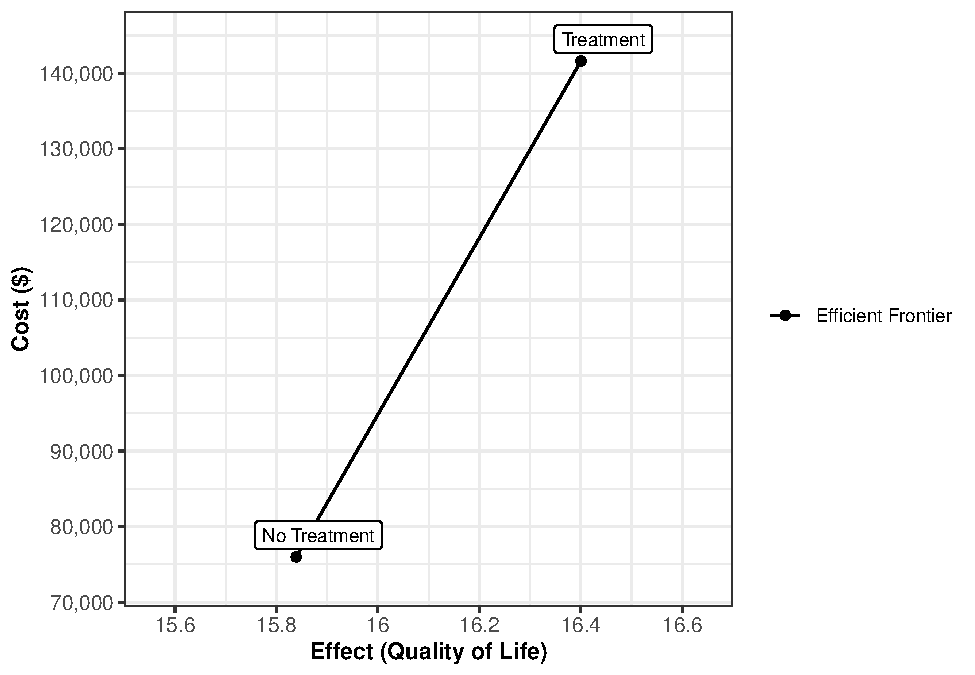
\includegraphics{markov_sick-sicker_tunnels_solutions_files/figure-latex/unnamed-chunk-18-1.pdf}

\end{document}
